\documentclass{article}
\usepackage{graphicx} % Required for inserting images
\usepackage{outlines}
\usepackage{svg}
\usepackage[hidelinks]{hyperref} % removal of green square
\usepackage{tikz}
\usetikzlibrary{positioning}
\usepackage[numbers]{natbib} % Use natbib instead of cite


\begin{filecontents}{inline.bib}



@misc{wcced2018,
  author = {WHO},
  title = {Cervical Cancer Elimination Initiative},
  howpublished = {\url{https://www.who.int/initiatives/cervical-cancer-elimination-initiative}},
  note = {Accessed: \today}
}

@misc{wcced2022,
  author = {WHO},
  title = {17 November is the Cervical Cancer Elimination Day of Action},
  howpublished = {\url{https://www.who.int/campaigns/cervical-cancer-elimination-day-of-action}},
  note = {Accessed: 24/06/2023}
}

@misc{mayo_hpv2023,
  author = {Mayo Clinic},
  title = {HPV infection - Diagnosis and treatment},
  howpublished = {https://www.mayoclinic.org/diseases-conditions/hpv-infection/diagnosis-treatment/drc-20351602},
  note = {Accessed: 24/06/2023}
}

@misc{mayo_cc2023,
  author = {Mayo Clinic},
  title = {Cervical cancer - Diagnosis and treatment},
  howpublished = {https://www.mayoclinic.org/diseases-conditions/cervical-cancer/diagnosis-treatment/drc-20352506},
  note = {Accessed: 24/06/2023}
}

@misc{whocpc2021,
  author = {WHO},
  title = {WHO guideline for screening and treatment of cervical pre-cancer lesions for cervical cancer prevention},
  howpublished = {https://www.who.int/news/item/06-07-2021-q-and-a-screening-and-treatment-cervical-pre-cancer-lesions-for-cervical-cancer-prevention},
  note = {Accessed: 24/06/2023}
}

@misc{pcf2023,
  author = {Prevent Cancer Fundation},
  title = {Global Grants},
  howpublished = {https://www.preventcancer.org/programs/our-global-reach/global-grants/},
  note = {Accessed: 24/06/2023}
}


@misc{esmo2023,
  author = {ESMO},
  title = {Major National Research Funds in Europe, North America, Asia and Australia},
  howpublished = {https://www.esmo.org/research/research-funding-opportunities/other-research-funding-opportunities/national-research-funds},
  note = {Accessed: 24/06/2023}
}


@misc{mobileodt2023,
  author = {mobileODT},
  title = {The MobileODT Single Visit Program},
  howpublished = {https://www.mobileodt.com/screen-treat-program/},
  note = {Accessed: 24/06/2023}
}


\end{filecontents}



%%%%%%%%%%
\title{Saving My Mother, One Screening at a Time  \\
---A WHO Cervical Cancer Elimination Day of Action in Somaliland (2023/11/17)}
\author{Dr. Tex Li-Hsing Chi, D.D.S., Ph.D.}
\date{\today}

\begin{document}


\begin{titlepage}
%    \centering

%\begin{center}
\hspace*{-0.7cm}%
\begin{tikzpicture} % tikzfigure
%\begin{minipage}[b]{1\linewidth}

\includesvg[height=3.0cm, distort=false]{Flag_of_the_Republic_of_China.svg}
\hspace{1.4cm}
%\includesvg[width=0.17\linewidth]{TMM_logo.svg}
%\hspace{3cm}
\includesvg[height=3.0cm, distort=false]{Flag_of_Somaliland.svg}
%\captionof{Figure}{xx}
%\end{minipage}
\end{tikzpicture}
    \vspace{2cm}
    
\centering
    {\Huge\bfseries Taiwan Medical Mission in the Republic of Somaliland \\
    \par } % \\
 %   Handbook\par}
    \vspace{1.5cm}
    %\hspace{4cm} 
    {\Large \today \par}

%\end{center}

\vspace{2.0cm}
%\includesvg[height=1.0cm, distort=false]{TMWH_logo_TAIPEI_vector.svg}
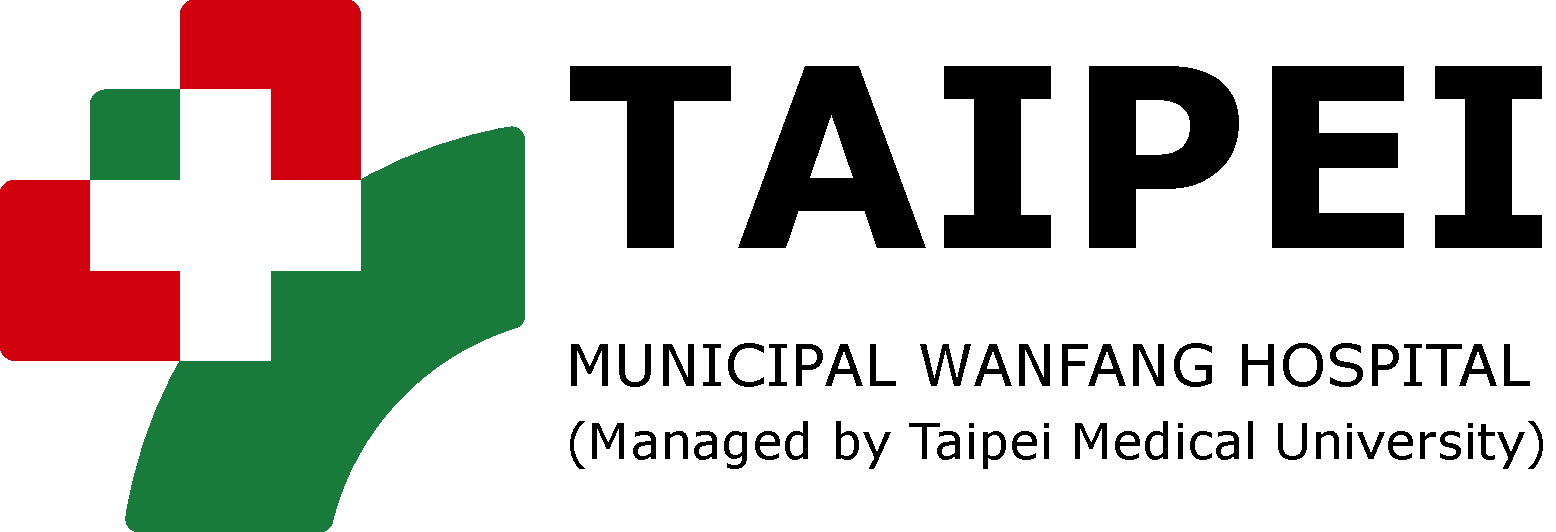
\includegraphics[height=1.5cm]{TMWH_logo_TAIPEI_vector.pdf}
\includesvg[height=1.5cm, distort=false]{Hargeisa_Group_Hospital_logo.svg}\\
\vspace{2.5cm}
\includesvg[height=5cm, distort=false]{TMM_logo.svg}
\hspace{0.5cm}
\includesvg[height=5cm, distort=false]{anti_CervicalCancer_logo.svg}
%\includegraphics[height=2cm]{WHA_WNW_Logo_CMYK-scaled-1.jpg}
\end{titlepage}



\maketitle

\section{Introduction}

The Cervical Cancer Elimination Day of Action is an annual event that takes place on November 17th. It marks the anniversary of the launch of the "Global Strategy to Accelerate the Elimination of Cervical Cancer" as a public health problem by the World Health Organization (WHO).

Cervical cancer is a preventable and curable disease, yet it remains the 4th most common form of cancer among women worldwide. In May 2018, the WHO Director-General announced a global call for action to eliminate cervical cancer\citep{wcced2018}, underscoring renewed political will to make elimination a reality and calling for all stakeholders to unite behind this common goal. In August 2020, the World Health Assembly adopted the Global Strategy for cervical cancer elimination. Now is the time to act to eliminate cervical cancer as a public health problem.
The Taiwan Medical Mission proposes a medical campaign called "WHO Cervical Cancer Elimination Day of Action"\citep{wcced2022} to be held at Hargeisa Group Hospital on November 17th, 2023.
Our hashtags are  \#GlowTeal and \#CervicalCancer.

Human papillomavirus (HPV) is a common transmitted infection that can cause cervical cancer in women. HPV infection often has no symptoms, so many people may not know they have it. There are many different types of HPV, some of which can cause cancer.

Cervical cancer screening can help detect abnormal cells in the cervix before they develop into cancer. The two main types of cervical cancer screening tests are the Pap test and the HPV DNA test. 
During a Pap test, a sample of cells is collected from the cervix and examined by cytologist for abnormalities.
During a Pap test, a sample of cells from the cervix is obtained and analyzed for abnormalities by a cytologist.
An HPV DNA test can identify high-risk HPV varieties that are most likely to cause cervical cancer.
These tests are advised for women aged 30 to 49.\citep{mayo_hpv2023, whocpc2021}.

If abnormal cells are detected during cervical cancer screening, further testing and treatment may be necessary. Treatment options for pre-cancerous lesions include cryosurgery, laser surgery, surgical removal, loop electrosurgical excision procedure (LEEP), and cold knife conization\citep{mayo_cc2023}. These treatments aim to remove abnormal cells before they develop into cancer.

%It is important for women to talk to their doctor about their cervical cancer screening options and to get screened regularly to help prevent cervical cancer.
We will propose using the "screen-triage-treat" approach via HPV DNA testing, which has been recognized by the WHO as the primary screening method for eliminating cervical cancer globally\citep{whocpc2021}.
This project will enable the HPV self-sampling initiative, a widely used HPV testing method, to discover best practices in low-resource service delivery.

\section{Objectives}
%%% *** why and rationale
The main objective of this project is to improve cervical cancer prevention and screening in Somaliland by implementing the 2021 WHO recommendation guideline, which includes HPV DNA testing. 
The project aims to achieve the following targets by 2030\citep{wcced2018}: 
\begin{outline} 
\1 Vaccination: 90\% of girls fully vaccinated with the HPV vaccine by the age of 15. 
\1 Screening: 70\% of women screened using a high-performance test, including HPV DNA test, by the age of 35, and again by the age of 45. 
\1 Treatment: 90\% of women with pre-cancer treated and 90\% of women with invasive cancer managed. \end{outline}


\section{Methods}
%%%% 
%\begin{outline}
%The campaign will include the following activities:
The campaign will implement several strategies to improve cervical cancer prevention and screening in Somaliland: 

\begin{outline} 
\1 In-person communication and information material at Hargeisa Group Hospital (HGH): This can include brochures, posters, A5-sized notes from hospital information system (HIS) at OPD, and other informational materials that explain the importance of cervical cancer screening, how to get screened with both HPV DNA test and Pap smear, and the benefits of vaccination against HPV. 
\1 Better recall through SMS (Telesom or Somtel) written in Somali languages: A system can be set up to send reminders to women through SMS. These reminders can include information about how to attend a screening, recall for further therapy in case with abnormal findings of HPV DNA test or Pap smear, and when their next screening is due.
\1 Incentives: People can be encouraged to attend screenings through free health checks, small gifts (like multivitamin tablets), recognition, or small rewards. 
%\1 Offering breast ultrasound and cervical cancer screening together during a screening campaign can provide women with the opportunity to have two important health screenings at the same time. 
\1 Verbal communication through seminars and workshops: Seminars and workshops can be organized to educate women about their risk of cancer and the importance of screening. 
\1 Screening approach
    \2 screen-treat method: Taking Pap smear, then follow or treat according to cytology result
    \2 screen-triage-treat (mobileODT)\citep{mobileodt2023} at once: It offers a full turnkey diagnostic and treatment program utilizing the HPV DNA rapid test, the EVAPro digital colposcope and the ThermoGlide, for thermocoagulation treatment of precancerous lesions.

\end{outline}

%%%%

\section{Sustainability} 
To ensure the sustainability of the project, several measures will be implemented: 

\begin{outline} 
\1 Collaboration with local organizations: Partnering with local organizations can help to ensure that the campaign is culturally sensitive and tailored to the needs of the local population. 
\1 Training of healthcare professionals: Training healthcare professionals on the importance of cervical cancer screening and how to perform HPV DNA tests and Pap smears can help to ensure that women receive high-quality care. 
\1 Regular follow-up: Regular follow-up with women who have attended screenings can help to ensure that they receive appropriate care if any abnormalities are detected. 
\1 Data collection and analysis: Collecting data on the number of women who attend screenings, the results of their tests, and any follow-up care they receive can help to evaluate the effectiveness of the campaign and identify areas for improvement. 
\1 Funding: Securing long-term funding for the campaign from organizations such as WHO\citep{wcced2018}, Prevent Cancer Foundation\citep{pcf2023}, or European Society for Medical Oncology (ESMO)\citep{esmo2023} can help to ensure its sustainability. 

\end{outline}

%%%
\section{Expected Outcomes}
The expected outcomes of this project include: 
\begin{outline} 
\1 Increased awareness about cervical cancer prevention among women in Somaliland. 
\1 Improved participation in cervical cancer screening among women in Somaliland. 
\1 Improved access to high-quality cervical cancer prevention services for women in Somaliland. \end{outline}

\section{Conclusion}


This project aims to improve cervical cancer prevention and screening in Somaliland by implementing evidence-based strategies that are tailored to the needs of the local population. 
By achieving its objectives, this campaign can contribute to eliminating cervical cancer as a public health problem in Somaliland.

%Summarize the benefits of implementing a PACS system with telemedicine support at HGH
%Reiterate the goals of TMM in delivering this project

%Vitamin D deficiency is a significant health situation among Somaliland women. By providing blood tests, bone density screening, and education on World Osteoporosis Day, we can help address this issue and improve the bone health of this population.
%In addition to the proposed project activities, we plan to explore the development of a wearable device that can be incorporated into hijab to increase artificial sun exposure. This device would use solar energy to power ultraviolet B LED lights, providing a safe and convenient way for Muslim women to improve their vitamin D levels.

%Postmenopausal osteoporosis is a bone disease that affects biological women after natural or surgical menopause. It is characterized by a progressive loss of bone tissue and density, increasing the risk of fracture. It is related to estrogen deficiency and increased follicle stimulating hormone, which play a role in the bone remodeling process. During the menopausal transition period, the drop in estrogen leads to more bone resorption than formation, resulting in osteoporosis.

%There are several ways postmenopausal women can improve their bone quality and quantity. One way is through weighted exercises, which can help maintain bone mineral density (BMD) in postmenopausal women and increase BMD of the spine and hip in women with osteopenia and osteoporosis. 

\bibliographystyle{plainnat} % Use plainnat instead of plain
\bibliography{inline,whd2023}


\end{document}


%%%% spared

\section{Draft Schedule}
An ENT campaign (e.g., operation for Tonsillitis) in Hargeisa, Somaliland, in August 2023:
\begin{outline}

	\1 (Briefing) On August 12 (Saturday), Dr. Hung will arrive one day ago and meet Dr. Omar, Dr. Hersi in Hargeisa, and the other local authorities and health officials to discuss the objectives and logistics of the campaign. They will also visit the Hargeisa Group Hospital (HGH) and inspect the facilities and equipment available for the surgery. They will review the list of patients Dr. Hersi screened and collected in July and select the most suitable candidates for the operation (a maximal of 40 patients).
	\1 (Surgery at HGH OT: August 14, 15) 
        \2 On August 14 (Monday) and August 15 (Tuesday), Dr. Hung and Hersi will perform the surgery on the selected patients at HGH with the assistance of local medical staff. They will also provide post-operative care and instructions to the patients and their families. They will monitor the recovery and outcomes of the surgery and document any complications or challenges. 
	\1 (Surgery or Debriefing)
        \2 On August 16 (Wednesday), they will also conduct a debriefing session with the local health authorities and HGH staff to share their feedback and recommendations for future campaigns.
\end{outline}


\section{Suggested Surgery}
Which kind of ENT surgery? by literature review:

Based on the web search results, some of the suggested ENT surgeries or diseases according to health statistics in Somaliland (or Somalia) are:

\begin{outline}

\1 *Tonsillitis, inflammation of the tonsils that can cause sore throat and fever.
\1 Cancer affecting the oral buccal mucosa, or lip in stage I without neck nodal disease clinically.
\1 Otosclerosis, a condition of the middle ear that causes hearing loss.
\1 Otitis media with effusion, also known as glue ear, in which the middle ear becomes blocked with fluid.
\1 Nasal polyps, benign growths in the nose that can cause obstruction and infection.

These are some of the common ENT problems that affect the population of Somaliland, especially children and elderly people. They may require surgical intervention or medical management depending on the severity and type of the condition.
\end{outline}


\section{Reference}
(1) Interpreting the Lancet surgical indicators in Somaliland: a cross-sectional study. https://bmjopen.bmj.com/content/10/12/e042968 Accessed 11/05/2023.
(2) ENT Department | Somali Sudanese specialized hospital. ENT Department | Somali Sudanese specialized hospital (ssshospital.so) Accessed 11/05/2023.

===

\section{Architecture of PACS for HGH}

The PACS architecture in HGH provides a standardized and efficient way to manage medical imaging data and ensure that it is accessible to healthcare professionals when and where it is needed.\\
The project involves the following architectures:

\begin{outline}
    \1 PACS will be installed in the radiology and pathology departments of HGH
        \2 Digital Imaging and Communications in Medicine, or DICOM, is the international standard for transmitting, storing, retrieving, printing, processing, and displaying information about medical imaging. It ensures that medical images meet quality standards and are used in most health organizations for diagnosis alongside clinical inputs. DICOM files usually include a large amount of additional data relevant to the core imaging information (pixel data which may be encoded in different ways). DICOM is essential to PACS.

        \2 PACS server: This server acts as a central repository for medical imaging data and is responsible for storing, retrieving, and transmitting DICOM files.
        \2 Connected to the PACS server are various medical imaging devices such as CT scanners, (MRI machines, future plans), and ultrasound machines. These devices generate medical images in DICOM format and transmit them to the PACS server for storage and retrieval.
        \2 Also connected to the PACS server are various desktop workstations and viewing devices (e.g., tablets and smartphones) used by healthcare professionals to access and view medical images, via 
            \3 Intranet connections
            \3 Wire or wireless connections
%These devices use specialized software to communicate with the PACS server and retrieve DICOM files for viewing.

        \2 Other systems can be integrated with the PACS server to provide a seamless flow of medical imaging data throughout HGH.
        \3 Hospital information systems (HIS) and Electronic health record (EHR) systems
        \3 Radiology information systems (RIS)
        \3 Pathology information systems (PIS)
        \3 Virtual autopsy or VIRTOPSY in Forensic Medicine. Virtual autopsy, also called postmortem imaging, is a non-invasive alternative to a traditional autopsy. It uses medical imaging techniques like computed tomography (CT) and magnetic resonance imaging (MRI) to see and record the internal structures of a dead person for forensic purposes. RIS and PIS can help with a virtual autopsy by managing and storing the medical imaging data that is made during the process. In forensic medicine, a virtual autopsy can give important information about the cause and manner of death, as well as other forensic data. It can be especially helpful when a standard autopsy can't be done or isn't wanted for religious or cultural reasons, or when the body has already started to break down. The virtual autopsy can also give more full and detailed information about the skeletal system and the major changes in the parenchyma.

%It is important to note that virtual autopsy is not intended to replace traditional autopsy, but rather to complement it by providing additional information that can aid in forensic investigations.

%Source: Conversation with Bing, 30/05/2023(1) The approach of virtual autopsy (VIRTOPSY) by ... - ScienceDirect. https://www.sciencedirect.com/science/article/pii/S2666225620300105 Accessed 30/05/2023.
%(2) A Practical Guide to Virtual Autopsy: Why, When and How. https://www.sciencedirect.com/science/article/pii/S0887217118300945 Accessed 30/05/2023.
%(3) Radiology in Forensic Medicine - Springer. https://link.springer.com/book/10.1007/978-3-319-96737-0 Accessed 30/05/2023.
        % the PIS (Pathology information system) automates samples, images, and reports and progressively incorporates PI (Pathology informatics), D-PATH (digital pathology), e-PATH (electronic pathology), PPH (Patho-pharmacology), virtual autopsy, and in general all types of translational research in the PMIS (pathology management information system).
        
\1 Telemedicine
    \2 DICOM images from ultrasound machines, or point-of-care ultrasound (POCUS) devices, could be sent from one place to another.
    
    \2 Teleradiology is the electronic transmission of DICOM images from one location to another. It has various applications, such as case referrals, consultation services, and education. In this project, we propose to use teleradiology to provide case consultation between Somaliland and Taiwan.

    \2 Telepathology is the electronic transmission of pathological images, usually derived from microscopic slide scanners, from one location to another. A DICOM converter should be applied to produce DICOM images from pathological images (e.g., MIRAX) which are acquired by microscopic slide scanners. It has various applications, such as case referrals, immunohistochemistry (IHC) services, and education. In this project, we propose to use telepathology to provide case consultation and IHC services between Somaliland and Taiwan. A workflow of telepathology includes:
%This includes images from various medical imaging modalities such as radiology, ultrasound, and pathology.


	\3 Dr. Omar, a pathologist in HGH, Somaliland, will share whole slide images through Vision Assist App.
 %will use the Vision Assist app to scan and export whole slide images of pathology in MIRAX format (one of the OpenSlide standard formats) from tissue samples obtained during surgery or biopsy. Then it could be converted as DICOM and uploaded in PACS.
    
%    \3 Dr. Omar will upload the images to PACS and share them with a pathologist in Taipei.
     %, Taiwan, who will review them using QuPath software (\url{https://qupath.readthedocs.io/en/0.4/docs/intro/installation.html}). Alternatively, the Taipei pathologist can use their preferred software viewer if it can read MIRAX files.

    \3 Dr. Omar and the Taipei pathologist will communicate via Webex Meetings (\url{https://www.webex.com/video-conferencing}), a free and secure online tool for video conferencing that allows screen sharing and annotation. They will do bi-weekly teleconsultations of digital pathology for referring cases and training on the job. They will discuss the diagnosis and treatment options based on the images and the clinical information. This is meant to assist in building up the pathology profession in Somaliland and make it easy for pathologists from Taiwan and Somaliland to work together.
    
    \3 If immunohistochemistry (IHC) is needed for precision diagnosis, Dr. Omar will send formalin-fixed paraffin-embedded (FFPE) tissue blocks to Taipei via DHL Medical Express, a reliable and fast courier service for medical specimens. The Taipei pathologist will perform the appropriate IHC process and share the results with Dr. Omar. The patient will be responsible for paying for IHC services and DHL fees.
% (\url{https://www.dhl.com/global-en/home/our-divisions/express/industry-sectors/life-sciences-and-healthcare.html})

\1 Last-mile delivery
    \2 PACS server is accessed by computer/tablet in HGH (reports and images)
    \2 RadiPush and PathoPush: an alarm system for critical diagnoses. It can help healthcare professionals quickly identify and respond to emergency or critical situations. This can improve patient outcomes and help to save lives in situations where timely intervention is critical.
    
        \3 RadiPush (reports through SMS): to give patients an alarm system when a diagnosis hits a certain level of danger. RadiPush focuses on radiology diagnoses that fit certain critical scenarios, like tension pneumothorax, airway compromise, and cardiac tamponade.

        \3 PathoPush (reports through SMS): to give patients an alarm system when a diagnosis hits a certain level of danger. PathoPush is all about finding out if someone has cancer.

 
\end{outline}

\clearpage
%%%%%%%%%%%%%%%
% tikzpicture
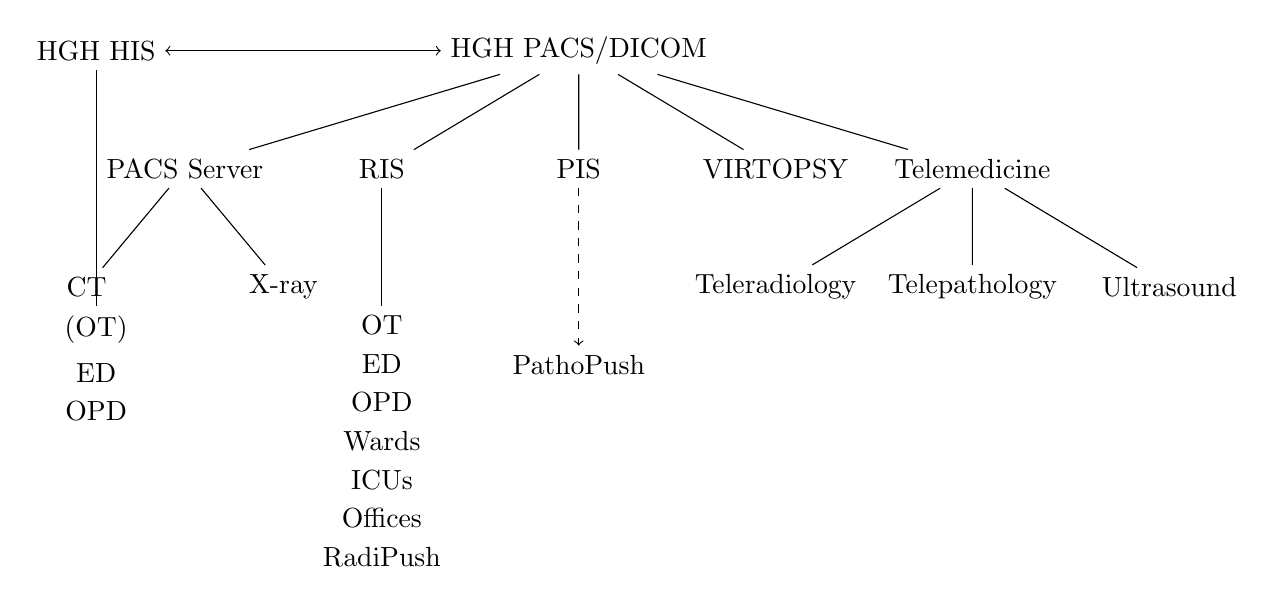
\begin{tikzpicture}[
    level 1/.style={sibling distance=25mm},
    level 2/.style={sibling distance=25mm},
    level 3/.style={sibling distance=20mm, level distance=40mm}]
%    level 4/.style={sibling distance=20mm, level distance=30mm},
%    level 5/.style={level distance=30mm},
%    level 6/.style={level distance=30mm},
%    level 7/.style={level distance=30mm},
%    level 8/.style={level distance=30mm}]
\node (his) {HGH HIS};
\node[below=30mm of his] (ot1) {(OT)};
\draw (his) -- (ot1);
\node[below=0mm of ot1] (ed1) {ED};
\node[below=0mm of ed1] (opd1) {OPD};
%\node[below=0mm of opd1] (wards1) {Wards};
%\node[below=0mm of wards1] (icus1) {ICUs};
%\node[below=0mm of icus1] (offices1) {Offices};
%\node[below=0mm of offices1] (radiPush1) {RadiPush};

\node[right=35mm of his] (pacs) {HGH PACS/DICOM} % ---
    child {node {PACS Server}
        child {node {CT}}
        child {node {X-ray}}}
    child {node (ris) {RIS}}
%        child[grow=down, edge from parent/.style={draw}] {node (ot) {OT}}
%        child[grow=down, edge from parent/.style={draw=none}] {node {ED}}
%        child[grow=down, edge from parent/.style={draw=none}] {node {OPD}}
%        child[grow=down, edge from parent/.style={draw=none}] {node {Wards}}
%        child[grow=down, edge from parent/.style={draw=none}] {node {ICUs}}
%        child[grow=down, edge from parent/.style={draw=none}] {node {Offices}}
%        child[grow=down, edge from parent/.style={draw=none}] {node {RadiPush}}}
    child {node (pis) {PIS}}
%        child {node {PathoPush}}}
    %child {node {HIS}}
    child {node {VIRTOPSY}}
    child {node {Telemedicine}
        child {node {Teleradiology}}
        child {node {Telepathology}}
        child {node {Ultrasound}}};
%\node[left=of pacs] (his) {HIS};
%\node[right=3cm of pacs] (his) {HIS};
\draw (his) edge[<->] (pacs);
\node[below=15mm of ris] (ot) {OT};
\draw (ris) -- (ot);
\node[below=0mm of ot] (ed) {ED};
\node[below=0mm of ed] (opd) {OPD};
\node[below=0mm of opd] (wards) {Wards};
\node[below=0mm of wards] (icus) {ICUs};
\node[below=0mm of icus] (offices) {Offices};
\node[below=0mm of offices] (radiPush) {RadiPush};

\node[below=20mm of pis] (pathopush) {PathoPush};
\draw[dashed, ->] (pis) -- (pathopush);




%\node [below of = Telemedicine] {Teleradiology}
%    child {node {Teleradiology}}
%    child {node {Telepathology}}
%    child {node {Ultrasound}};
%\node [below of = HGH PACS] {Last-mile Delivery}
%    child {node {RadiPush}}
%    child {node {PathoPush}};
%\node [below of = {PACS Server}] {DICOM compliance}
\end{tikzpicture}
% You can also customize the diagram by changing the values of sibling distance and level in the code.

The hierarchy diagram of PACS (DICOM compliance): It includes PACS server, medical imaging, CT scanners, ultrasound machines, hospital information system, radiology information system, pathology information system, virtual autopsy (VIRTOPSY), telemedicine, teleradiology, telepathology, RadiPush, and PathoPush.
Due to the vast spread of departments and system stability, the HGH intranet system should ideally be connected over a fiberoptic network.
%%%%%%%%%%%%%%
\clearpage